% ---------------------------------------------
% Alle Abbildungen 'images/' in Latex speichern 
%     * 'archiv/Pics-files.tex' 
%     * Bildgröße: 0.80/1 
% ju 05-Jun-2022 Pics-files.tex
% ---------------------------------------------
%
%\section{01_Anordnung-der-Nockenwelle_Skizze}
%
%01_Anordnung-der-Nockenwelle_Skizze (\autoref{fig:01_Anordnung-der-Nockenwelle_Skizze}).% Referenz
%
\begin{figure}[!hb]% hier: !hb
    \centering
  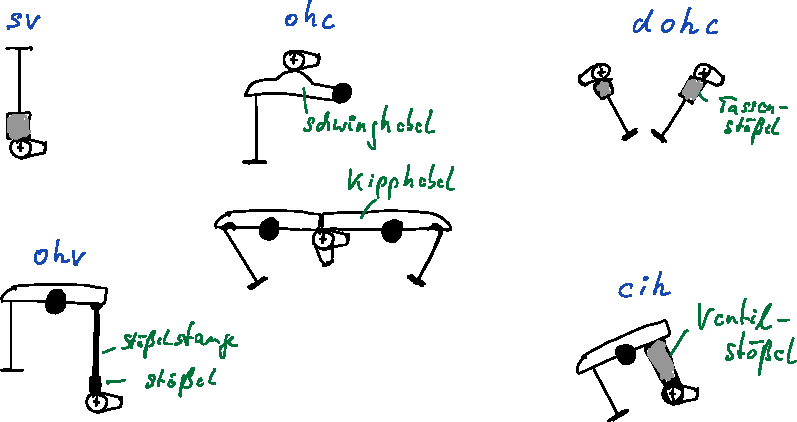
\includegraphics[width=.80\textwidth]{images/01_Anordnung-der-Nockenwelle_Skizze.pdf}%
  \caption{01_Anordnung-der-Nockenwelle_Skizze}%\label{fig:01_Anordnung-der-Nockenwelle_Skizze}%% anpassen
\end{figure}

%\newpage
%\section{02_Nockenformen_Skizze}
%
%02_Nockenformen_Skizze (\autoref{fig:02_Nockenformen_Skizze}).% Referenz
%
\begin{figure}[!hb]% hier: !hb
    \centering
  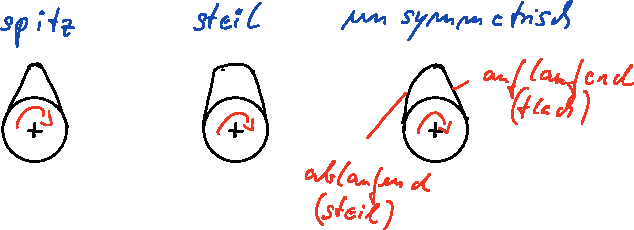
\includegraphics[width=.80\textwidth]{images/02_Nockenformen_Skizze.pdf}%
  \caption{02_Nockenformen_Skizze}%\label{fig:02_Nockenformen_Skizze}%% anpassen
\end{figure}

%\newpage
%\section{03_Arten-von-Ventilbetaetigung_Skizze}
%
%03_Arten-von-Ventilbetaetigung_Skizze (\autoref{fig:03_Arten-von-Ventilbetaetigung_Skizze}).% Referenz
%
\begin{figure}[!hb]% hier: !hb
    \centering
  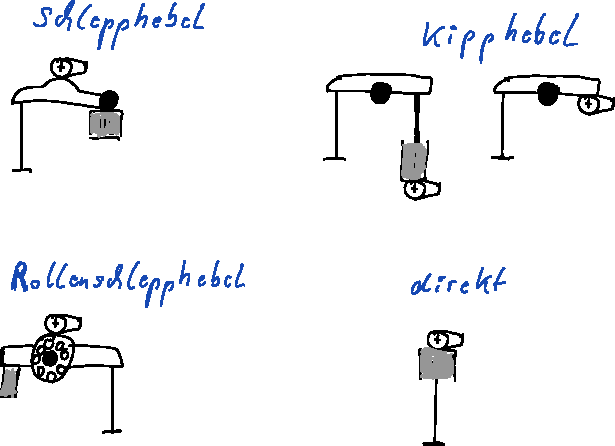
\includegraphics[width=.80\textwidth]{images/03_Arten-von-Ventilbetaetigung_Skizze.pdf}%
  \caption{03_Arten-von-Ventilbetaetigung_Skizze}%\label{fig:03_Arten-von-Ventilbetaetigung_Skizze}%% anpassen
\end{figure}

%\newpage
%\section{04_Ventilspielausgleich_Skizze}
%
%04_Ventilspielausgleich_Skizze (\autoref{fig:04_Ventilspielausgleich_Skizze}).% Referenz
%
\begin{figure}[!hb]% hier: !hb
    \centering
  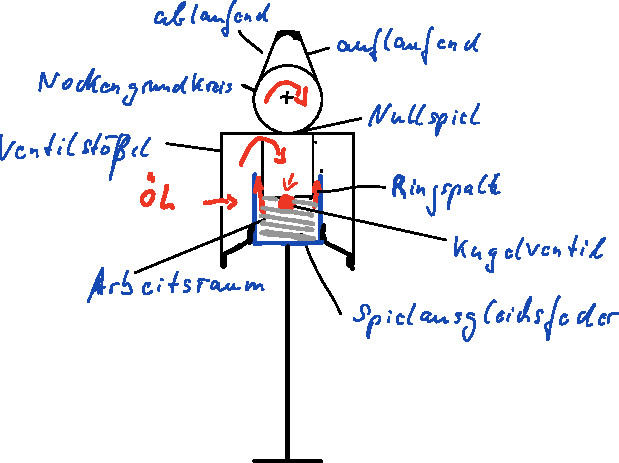
\includegraphics[width=.80\textwidth]{images/04_Ventilspielausgleich_Skizze.pdf}%
  \caption{04_Ventilspielausgleich_Skizze}%\label{fig:04_Ventilspielausgleich_Skizze}%% anpassen
\end{figure}

%\newpage
%\section{05_Dreiventiltechnik_Skizze}
%
%05_Dreiventiltechnik_Skizze (\autoref{fig:05_Dreiventiltechnik_Skizze}).% Referenz
%
\begin{figure}[!hb]% hier: !hb
    \centering
  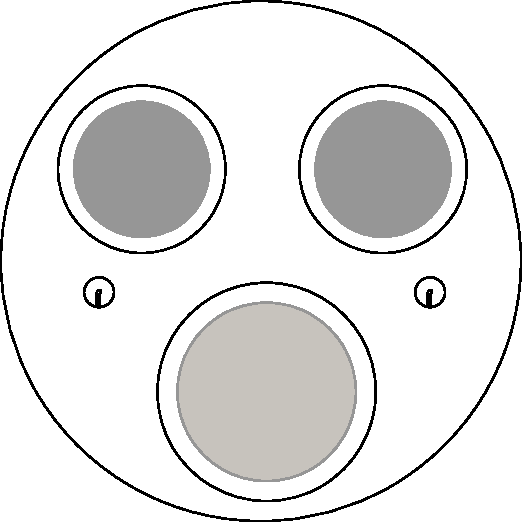
\includegraphics[width=.80\textwidth]{images/05_Dreiventiltechnik_Skizze.pdf}%
  \caption{05_Dreiventiltechnik_Skizze}%\label{fig:05_Dreiventiltechnik_Skizze}%% anpassen
\end{figure}

%\newpage
%\section{Mischungs-Luftverhaeltnis}
%
%Mischungs-Luftverhaeltnis (\autoref{fig:Mischungs-Luftverhaeltnis}).% Referenz
%
\begin{figure}[!hb]% hier: !hb
    \centering
  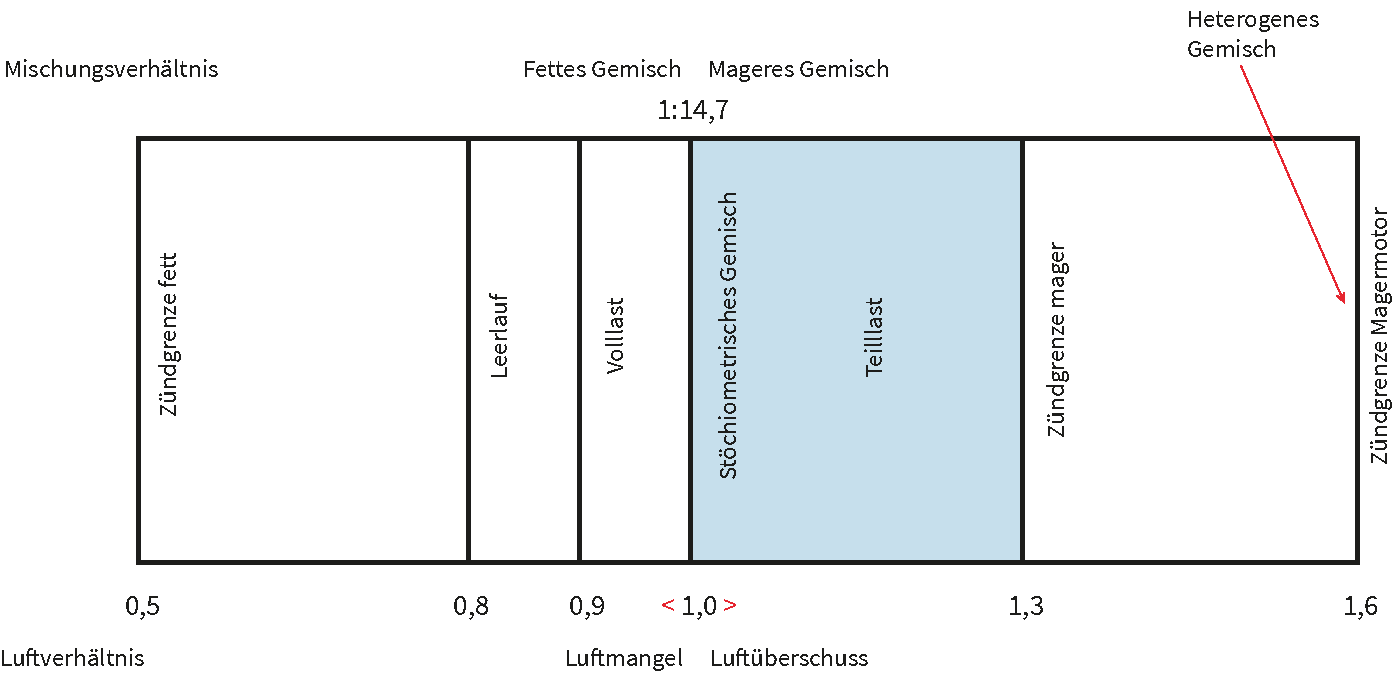
\includegraphics[width=.80\textwidth]{images/Mischungs-Luftverhaeltnis.pdf}%
  \caption{Mischungs-Luftverhaeltnis}%\label{fig:Mischungs-Luftverhaeltnis}%% anpassen
\end{figure}

%\newpage
%\section{Motorzylinder_v2}
%
%Motorzylinder_v2 (\autoref{fig:Motorzylinder_v2}).% Referenz
%
\begin{figure}[!hb]% hier: !hb
    \centering
  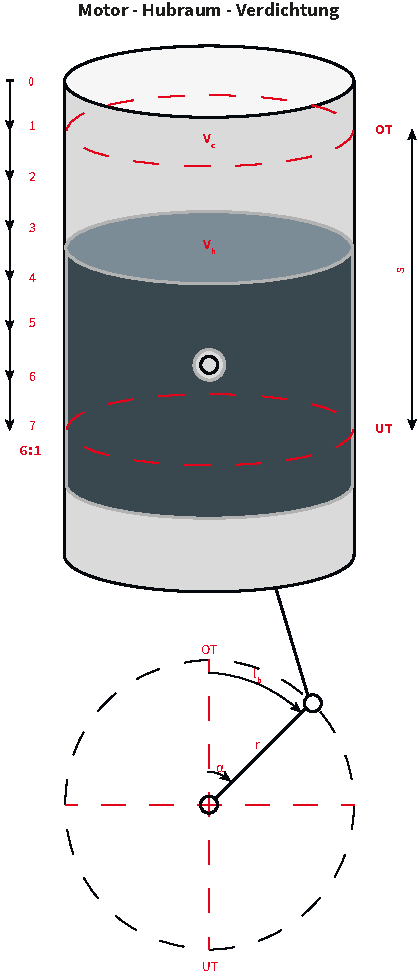
\includegraphics[width=.80\textwidth]{images/Motorzylinder_v2.pdf}%
  \caption{Motorzylinder_v2}%\label{fig:Motorzylinder_v2}%% anpassen
\end{figure}

%\newpage
